\documentclass[a4paper,english,12pt,appendix,twoside]{article}
%%
%% Formats and Defs
%%
% !TeX spellcheck = en_US

% Packages
\usepackage{epsf}
\usepackage{epsfig}
\usepackage[T1]{fontenc}
\usepackage{latexsym}
\usepackage{ucs}
\usepackage[utf8x]{inputenc}
\usepackage{float}
\usepackage[usenames]{color}
\usepackage{newcent}
\usepackage{graphicx}
\usepackage{setspace}
\onehalfspacing
\usepackage[numbers]{natbib}
\usepackage{setspace}
\usepackage{url}
\usepackage{eso-pic}
\usepackage{listings}
\usepackage{verbatim}
\usepackage{moreverb}
\usepackage{microtype}
\usepackage[noauto]{chappg}
\usepackage{lmodern}
\usepackage{appendix}
\usepackage{libertine}


\renewcommand{\lstlistingname}{Example}
\renewcommand{\lstlistlistingname}{List of Examples}

% Section rules
\usepackage{sectsty}
\usepackage{times}

% Bookmarks

% black references
%\usepackage[pdfborder={0 0 0}]{hyperref} 

% red references
\usepackage[colorlinks=true,linkcolor = blue]{hyperref}

% Colors
\definecolor{light-gray}{gray}{0.95}
\definecolor{gray}{gray}{0.2}
\definecolor{blue}{rgb}{0,0,1}
\definecolor{red}{rgb}{1,0,0}
\definecolor{green}{rgb}{0,0.69,0}
\definecolor{yellow}{rgb}{1,0.35,0}

% Listings settings
\lstdefinelanguage{lua}{
	morekeywords={and,break,do,else,elseif,end,false,for,function,if,in,local,nil,not,or,repeat,return,then,true,until,while},
	morekeywords={[2]arg,assert,collectgarbage,dofile,error,_G,getfenv,getmetatable,ipairs,load,loadfile,loadstring,next,pairs,pcall,print,rawequal,rawget,rawset,select,setfenv,setmetatable,tonumber,tostring,type,unpack,_VERSION,xpcall},
	morekeywords={[2]coroutine.create,coroutine.resume,coroutine.running,coroutine.status,coroutine.wrap,coroutine.yield},
	morekeywords={[2]module,require,package.cpath,package.load,package.loaded,package.loaders,package.loadlib,package.path,package.preload,package.seeall},
	morekeywords={[2]string.byte,string.char,string.dump,string.find,string.format,string.gmatch,string.gsub,string.len,string.lower,string.match,string.rep,string.reverse,string.sub,string.upper},
	morekeywords={[2]table.concat,table.insert,table.maxn,table.remove,	table.sort},
	morekeywords={[2]math.abs,math.acos,math.asin,math.atan,math.atan2,math.ceil,math.cos,math.cosh,math.deg,math.exp,math.floor,math.fmod,math.frexp,math.huge,math.ldexp,math.log,math.log10,math.max,math.min,math.modf,math.pi,math.pow,math.rad,math.random,math.randomseed,math.sin,math.sinh,math.sqrt,math.tan,math.tanh},
	morekeywords={[2]io.close,io.flush,io.input,io.lines,io.open,io.output,io.popen,io.read,io.tmpfile,io.type,io.write,file:close,file:flush,file:lines,file:read,file:seek,file:setvbuf,file:write},
	morekeywords={[2]os.clock,os.date,os.difftime,os.execute,os.exit,os.getenv,os.remove,os.rename,os.setlocale,os.time,os.tmpname},
	keywordstyle=\color{blue}\normalfont,
	ndkeywordstyle=\color{black}\normalfont,
	commentstyle=\color{red}\ttfamily,
	stringstyle=\color{green}\ttfamily,
	identifierstyle=\color{gray},
	sensitive=true,
	morecomment=[l]{--},
	morecomment=[s]{--[[}{]]--},
	morestring=[b]",
	morestring=[d]',
	backgroundcolor=\color{white}, 
	frame=single, 
	frameround=ffff,
	captionpos=b,
	basicstyle=\scriptsize
}

\lstdefinelanguage{nil}{
  identifierstyle=\color{gray},
  sensitive=false,
  columns=flexible,
  backgroundcolor=\color{white}, 
  frame=single, 
  frameround=ffff,
  captionpos=b
}

\lstdefinelanguage{javascript}{
  keywords={typeof, new, true, false, catch, function, return, null, catch, switch, var, if, in, while, do, else, case, break},
  ndkeywords={class, export, boolean, throw, implements, import, this},
  sensitive=false,
  comment=[l]{//},
  morecomment=[s]{/*}{*/},
  morestring=[b]',
  morestring=[b]",
  keywordstyle=\color{blue}\normalfont,
	ndkeywordstyle=\color{black}\normalfont,
	commentstyle=\color{red}\ttfamily,
	stringstyle=\color{green}\ttfamily,
	identifierstyle=\color{gray},
	backgroundcolor=\color{white}, 
	frame=single, 
	frameround=ffff,
	captionpos=b,
	basicstyle=\scriptsize
}

\lstdefinestyle{color}
	{identifierstyle=\color{green}\bfseries, commentstyle=\color{yellow}\bfseries, stringstyle=\color{blue}, keywordstyle=\color{red}\bfseries,morecomment=[l]{\#}}

\lstset{postbreak=\small>>\space,prebreak=\small>>,breakindent=13pt,breaklines=true,inputencoding=utf8x,tabsize=2,showtabs=false,tab=$\to$,style=color,basicstyle=\footnotesize\ttfamily\normalfonts,frame=lines,frameround=tttt}

% Figures settings
%\usepackage[small,normal,up]{caption2}
%\renewcommand{\captionfont}{\small\itshape}
%\graphicspath{{figures/}}

%
% this makes list spacing much better.
%
\newenvironment{my_itemize}{
\begin{itemize}
  \setlength{\itemsep}{1pt}
  \setlength{\parskip}{0pt}
  \setlength{\parsep}{0pt}}{
\end{itemize}
}

\newenvironment{my_enumerate}{
\begin{enumerate}
  \setlength{\itemsep}{1pt}
  \setlength{\parskip}{0pt}
  \setlength{\parsep}{0pt}}{
\end{enumerate}
}

\newcommand{\emptyitem}{\item[]}
\newcommand{\myitem}{\item[$-$]}

%Font settings
%\makeatletter
%\renewcommand{\paragraph}{\@startsection{paragraph}{4}		
%{0ex}%
%{-3.25ex plus -1ex minus -0.2ex}%
%{1.5ex minus 0.2ex}%
% {\normalfont\normalsize\bfseries}}

\makeatother


\stepcounter{secnumdepth}
\stepcounter{tocdepth}

\setcounter{secnumdepth}{3}
\setcounter{tocdepth}{3}
%% SET THE LANGUAGE DEFINED
\newif\ifenglish
\englishfalse %% to use slovak template change the command to \englishfalse
%%
%\usepackage[slovak]{babel}
%\usepackage[IL2]{fontenc}                                                   

\let\oldsection\section
\def\section{\cleardoublepage\oldsection}
\usepackage{emptypage}
%\usepackage[a4paper,left=1in,right=1in,top=1in,bottom=1in,footskip=.25in]{geometry}
\usepackage[a4paper, bindingoffset=12mm]{geometry}
\usepackage{algorithm}
\usepackage{algpseudocode}

\usepackage{listings}
\usepackage{color} %red, green, blue, yellow, cyan, magenta, black, white
\definecolor{mygreen}{RGB}{28,172,0} % color values Red, Green, Blue
\definecolor{mylilas}{RGB}{170,55,241}
\lstset{language=Java,
	basicstyle=\ttfamily,
	showspaces=false,
	numbers=left,
}


\makeatletter
\def\BState{\State\hskip-\ALG@thistlm}
\makeatother

\floatname{algorithm}{Algoritmus}
\renewcommand{\algorithmicrequire}{\textbf{Vstupy: }}
\renewcommand{\algorithmicensure}{\textbf{Výstupy: }}
\renewcommand{\listalgorithmname}{Zoznam algoritmov}

\makeatletter
\renewcommand\subparagraph{\@startsection{subparagraph}{5}{\z@}%
	{-3.25ex\@plus -1ex \@minus -.2ex}%
	{0.0001pt \@plus .2ex}%
	{\normalfont\normalsize\bfseries}}
\makeatother

\usepackage[nottoc,notlof,notlot]{tocbibind}
\usepackage{tocloft}

\renewcommand\cftaftertoctitle{\par\noindent\hrulefill\par}
\renewcommand{\cftsecleader}{\cftdotfill{\cftdotsep}}


%%%%%%%%%%%%%%%%%%%%%%%%%%%%%%%%%%%%%%%%%%%%%%%%%%%%%%%%%%%%%%%%%%%%%%%%%%%%%%%%%%%%%%%%

%-------definitions-----
\newcommand{\Unisk}{Slovenská Technická Univerzita v Bratislave}
\newcommand{\Uni}{Slovak University of Technology in Bratislava}
\newcommand{\Facultysk}{Fakulta informatiky a informačných technológií}
\newcommand{\Faculty}{Faculty of informatics and information technologies}
\newcommand{\Thesis}{Master's thesis}
\newcommand{\Thesissk}{Diplomová práca}
\newcommand{\Author}{Name Surname} 
\newcommand{\Title}{Title English}
\newcommand{\Titlesk}{Title Slovak}
\newcommand{\Supervisor}{Supervisor's name}
\newcommand{\Decl}{Declaration}
\newcommand{\Declsk}{Čestné prehlásenie}
\newcommand{\Thanks}{Special thanks}
\newcommand{\Thankssk}{Poďakovanie}
\newcommand{\Superv}{Supervisor:}
\newcommand{\Supervsk}{Vedúci práce:}
\newcommand{\Place}{Institute of computer engineering and applied informatics}
\newcommand{\Placesk}{Ústav počítačového inžinierstva a aplikovanej informatiky}
\newcommand{\Year}{2017}
\newcommand{\Month}{May }
\newcommand{\Monthsk}{Máj }
\newcommand{\FIIT}{FIIT-XXXX-XXXXX}
\newcommand{\Field}{9.2.1 Informatics}
\newcommand{\Fieldsk}{9.2.1 Informatika}
\newcommand{\Program}{Informatics}
\newcommand{\Programsk}{Informatika}


%%
%% DON'T TOUCH
%%
%% PDF meta-data 
\hypersetup{%
pdftitle={\Title},%
pdfauthor={\Author},%
pdfkeywords={key words},%
}%

%%%%%%%%%%%%%%%%%%%%%%%%%%%%%%%%%%%%%%%%%%%%%%%%%%%%%%%%%%%%%%%%%%%%%%%%%%%%%%%%%%%%%%%%
%\usepackage{fancyhdr}

%\pagestyle{fancy}
%\pagestyle{fancy}
%\fancyhf{}
%\renewcommand{\subsectionmark}[1]{\markright{#1}}

%\fancyhead[R]{\rightmark}

%\renewcommand{\headrulewidth}{1pt}
\setcounter{tocdepth}{4}
\setcounter{secnumdepth}{4}
\makeatletter



\@addtoreset{paragraph}{subsubsection}
\makeatother
\usepackage{amsmath}
\usepackage{amssymb}
\usepackage{indentfirst}
\usepackage{physics}
%\usepackage{geometry}
\usepackage{lmodern}
\usepackage{lipsum}

\ifenglish
	\usepackage[english]{babel}                                               
	\usepackage[figurename=Fig.]{caption}
	\renewcommand{\captionfont}{\small\itshape}
	\graphicspath{{figures/}}
	\captionsetup[figure]{labelfont=normal,textfont=it}
	\addto\captionsenglish{% Replace "english" with the language you use
		\renewcommand{\contentsname}%
		{Table of contents}%
	}
\else
	\usepackage[slovak]{babel}                                               
	\usepackage[figurename=Obr.]{caption}
	\renewcommand{\captionfont}{\small\itshape}
	\graphicspath{{figures/}}
	\captionsetup[figure]{labelfont=normal,textfont=it}
	\addto\captionsenglish{% Replace "english" with the language you use
		\renewcommand{\contentsname}%
		{Obsah}%
	}
\fi



\begin{document}
\lstset{language=Matlab,%
	%basicstyle=\color{red},
	breaklines=true,%
	morekeywords={matlab2tikz},
	keywordstyle=\color{blue},%
	morekeywords=[2]{1}, keywordstyle=[2]{\color{black}},
	identifierstyle=\color{black},%
	stringstyle=\color{mylilas},
	commentstyle=\color{mygreen},%
	showstringspaces=false,%without this there will be a symbol in the places where there is a space
	numbers=none,%
	numberstyle={\tiny \color{black}},% size of the numbers
	numbersep=9pt, % this defines how far the numbers are from the text
	emph=[1]{for,end,break},emphstyle=[1]\color{red}, %some words to emphasise
	%emph=[2]{word1,word2}, emphstyle=[2]{style},    
}

\urlstyle{same}

% !TeX spellcheck = <none>
\begin{center}
\thispagestyle{empty}


\ifenglish
	{\Large \bf \Uni}\\[\baselineskip]
	{\large \Faculty}
\else
	{\Large \bf \Unisk}\\[\baselineskip]
	{\large \Facultysk}
\fi

\noindent\makebox[\linewidth]{\rule{\textwidth}{1pt}} 


\hspace{0.5cm}

{\large \bf \FIIT}\\
\vspace*{4.5cm}
{\Large \Author}\\[\baselineskip]
\ifenglish
	{\huge \bf \Title}\\[\baselineskip]
	{\large \Thesis}\\
\else
	{\huge \bf \Titlesk}\\[\baselineskip]
	{\large \Thesissk}\\
\fi
\end{center}
\vspace{7.4cm}
\ifenglish
	{\bf \Superv} \Supervisor \\
	\\
	\Month    \Year
\else
	{\bf \Supervsk} \Supervisor \\
	\\
	\Monthsk    \Year
\fi

%%
%% Title Page
%%
\begin{center}
\newpage
\thispagestyle{empty}

\ifenglish
	{\Large \bf \Uni}\\[\baselineskip]
	{\large \Faculty}
\else
	{\Large \bf \Unisk}\\[\baselineskip]
	{\large \Facultysk}
\fi


\noindent\makebox[\linewidth]{\rule{\textwidth}{1pt}} 


\hspace{0.5cm}

{\large \bf \FIIT}\\
\vspace*{4.5cm}
{\Large \Author}\\[\baselineskip]
\ifenglish
	{\huge \bf \Title}\\[\baselineskip]
	{\large \Thesis}\\
\else
	{\huge \bf \Titlesk}\\[\baselineskip]
	{\large \Thesissk}\\
\fi

\end{center}
\vspace{4.9cm}
\ifenglish
	{\bf Degree course:} \hspace*{1.4cm} \Program\\ 
	{\bf Field of study:}  \hspace*{1.6cm}\Field\\
	{\bf Place of elaboration:}  \hspace*{.5cm}\Place,\\ 
	\hspace*{4.4cm}FIIT STU, Bratislava \\
	{\bf \Superv}  \hspace*{2cm} \Supervisor \\ \\
	\Month    \Year
\else
	{\bf Štúdijný program:}  \hspace*{0.6cm} \Programsk\\ 
	{\bf Študijný odbor:}  \hspace*{1.1cm} \Fieldsk\\
	{\bf Miesto vypracovania:}  \hspace*{0.1cm} \Placesk,\\
	\hspace*{4.2cm}FIIT STU, Bratislava \\
	{\bf \Supervsk}  \hspace*{1.5cm} \Supervisor \\ \\
	\Monthsk    \Year
\fi

\pagenumbering{gobble}
\newpage\null\thispagestyle{empty}\newpage
%%
%% Declaration
%%

\newpage
\thispagestyle{plain}
\vspace*{13cm} 
\begin{large}
\noindent
%\textbf{DECLARATION} \\
\textbf{ČESTNÉ PREHLÁSENIE} \\
\end{large}
\noindent
Čestne prehlasujem, že predloženú bakalársku prácu som vypracoval samostatne pod vedením
Ing. Mareka Jakaba a uviedol v zozname literatúry všetky použité odborné zdroje.\\
\vspace*{0.5cm}\\
V Bratislave, 9.5.2017
\hspace*{7cm}............................\\
\hspace*{10.8cm} \Author
\newpage\null\thispagestyle{empty}\newpage

%%
%% Thanks
%%
\newpage
\thispagestyle{plain}
\vspace*{14cm} 
\noindent
\begin{center}
	\ifenglish
		{\large\textbf{\Thanks}} \\
	\else
		{\large\textbf{\Thankssk}} \\
	\fi
\end{center}

\noindent
Moje poďakovanie patrí najmä vedúcemu práce, ... , za jeho ľudský prístup, ochotu, odborné vedenie, metodickú pomoc a cenné rady, ktoré mi poskytol počas jej vypracovania. \\ \\
\noindent
Osobitné poďakovanie patrí mojim rodičom a mojim najbližším, za ich podporu, pomoc a vytvorenie podmienok pre vypracovanie bakalárskej práce.

\vspace*{0.7cm}
\noindent
\hspace{11.2cm}\Author
%\newpage\null\thispagestyle{empty}\newpage
%%
%% Anotation
%%

\newpage
\thispagestyle{plain}
%\begin{center}
%	{\small Slovenská Technická Univerzita v Bratislave}\\%[\baselineskip]
%	{\small \bf \uppercase {Fakulta informatiky a informaČnÝch technológií}}	
%	\noindent\makebox[\linewidth]{\rule{\textwidth}{1pt}}
%\end{center}

\noindent
{\huge\bf Anotácia}\\[\baselineskip]
\noindent 
\MakeUppercase{\Unisk}

\vspace*{.2cm}
\noindent
\MakeUppercase{\Facultysk}

\vspace*{.2cm}
\noindent
Študijný program: \hspace*{1.9cm} \Programsk

\vspace*{.7cm}
\noindent
Autor: \hspace*{3.9cm} \Author

\vspace*{.2cm}
\noindent
\Thesissk:\hspace*{2.2cm}\Titlesk

\vspace*{.2cm}
\noindent
Vedúci bakalárskej práce:\hspace*{.9cm}\Supervisor

\vspace*{.2cm}
\noindent
\Monthsk \Year
\noindent

\vspace*{2cm}
\noindent
\lipsum[1]
\newpage\null\thispagestyle{empty}\newpage


\thispagestyle{plain}
%\begin{center}
%	{\small Slovak University of Technology in Bratislava}\\%[\baselineskip]
%	{\small \bf \uppercase {Faculty of Informatics and Information Technologies}}	
%	\noindent\makebox[\linewidth]{\rule{\textwidth}{1pt}}
%\end{center}

\noindent
{\huge \bf Annotation}\\[\baselineskip]
\noindent
\noindent 
\MakeUppercase{\Uni}

\vspace*{.2cm}
\noindent
\MakeUppercase{\Faculty}

\vspace*{.2cm}
\noindent
Degree course: \hspace*{2.5cm} \Program

\vspace*{.7cm}
\noindent
Author: \hspace*{3.8cm}\Author

\vspace*{.2cm}
\noindent
\Thesis:\hspace*{2.6cm}\Title

\vspace*{.2cm}
\noindent
\Superv\hspace*{3.3cm}\Supervisor

\vspace*{.2cm}
\noindent
\Month \Year
\noindent

\vspace*{2cm}
\noindent
\lipsum[1]
\newpage\null\thispagestyle{empty}\newpage

%%
%% Contents
%%

\pagenumbering{roman}
\setcounter{page}{13}
%\pagestyle{empty}
\tableofcontents{}
%%
%% Lists
%%
 \newpage\null\thispagestyle{empty}\newpage
% List of Figures
% \listoffigures  
% \newpage
% List of Tables
% \listoftables
%\newpage

%\listofalgorithms
%\addtocontents{loa}{\def\string\figurename{Algoritmus}}
%\newpage\null\thispagestyle{empty}\newpage

%%
%% Clear Page And Set New Page Counter
%%
\clearpage
\pagenumbering{arabic}
\setcounter{page}{1}

\sectionfont{\sectionrule{0pt}{0pt}{-2ex}{0.5pt}}


%%
%% Introduction
%%
\newpage
\section{INtro}
%Sem niečo doplniť...fsfgrsdddd

%%
%% analysis
%%
\newpage

\section{Analýza problematiky}
\lipsum[3]

\subsection{Podsekcia 1}
\lipsum 

Segmentácia obrazu sa v dnešnej dobe využíva veľmi často v medicíne napr. pri snímkach mozgu \cite{5}, pri detekcií objektov, pri rozpoznávaní tváre \cite{6} a v neposlednom rade pri vyhľadávaní snímok na základe obsahu \cite{7}.

\subsubsection{Podsekcia 2}
Zoznam:
\begin{my_itemize}
	\item Položka 1
	\item Položka 2
\end{my_itemize}

\paragraph{Podsekcia 3}
\lipsum[1]

\begin{figure}[H]
	\begin{center}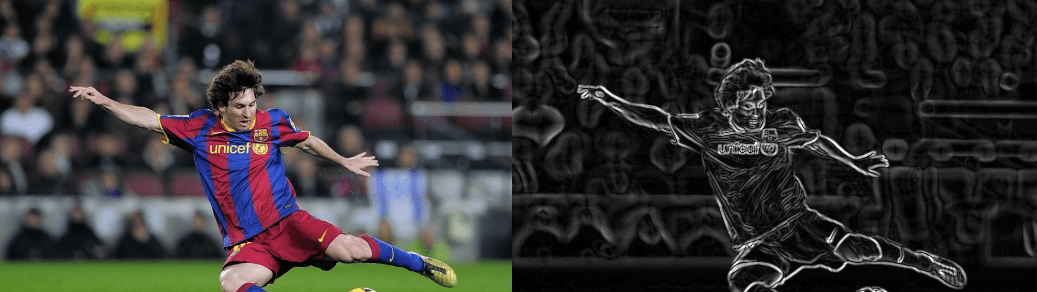
\includegraphics[scale=0.35]{figure3}\end{center}
	\caption[Sobel operátor]{Ukážka pred a po aplikácií Sobel operátora pri detekcií hrán\footnotemark 
		 
	}\label{f3}
\end{figure}
\footnotetext{Zdroj: WeekMedia, \href{http://opencvpython.blogspot.sk/2012/06/image-derivatives-sobel-and-scharr.html}{Abid Rahman K}}

\lipsum[1]

\paragraph{Podsekcia 3} \label{podobnost}

S algoritmom prichádza funkcia energie $E(s)$, ktorá ohodnocuje kvalitu špecifického rozdelenia obrazu a má tvar:
\begin{equation} \label{ener}
	E(s) = H(s) + \gamma G(s)
\end{equation}


%%
%% design
%%
\newpage
\section{Návrh}
\lipsum[1]
\subsection{Podsekcia 1}
\lipsum \dots

%%
%% implementation
%%
\newpage
\section{Implementácia}
\lipsum[1]

\subsection{Podsekcia 1} \label{iclass}
\noindent
\lipsum[1]

\begin{algorithm}[H]
	\small
	\caption{Načítanie údajov}\label{kinect}
	\algorithmicrequire $depthMat$, $colorMat$\\
	\algorithmicensure $depthMat$, $colorMat$
	
	\begin{algorithmic}[1]
		\Procedure{GetMappedColorData}{}
		\If {\textbf{getFrame}($frame$) = $success$}
		\State \textbf{mapData}($frame$, $mapped$)
		\If {\textbf{getColor}($frame$, $colorFrame$) = $success$}
		\State \textbf{copyFrameData}($colorFrame$, $colorData$)
		\For {$i<$\textbf{width}($color$)}
		\For {$j<$\textbf{height}($color$)}
		\State $depthSpacePoint \gets mapped[i][j]$
		\If {\textbf{visible}($depthSpacePoint$) $\not= success$}
		\State $depthMat[i][j]\gets -1$
		\Else
		\State $index\gets$ \textbf{getIndex}($depthSpacePoint$)
		\State $depthMat[i][j]\gets depthData[index]$
		\EndIf
		\State $colorMat[i][j]\gets colorData[i][j]$
		\EndFor
		\EndFor
		\EndIf
		\EndIf
		\EndProcedure
	\end{algorithmic}
\end{algorithm}
\noindent
V prvom pseudokóde so vstupnými a výstupnými parametrami typu \textbf{Mat} (typ reprezentujúci maticu definovaný v OpenCV) sme použili následovné metódy: \dots

%%
%% test
%%
%\newpage
\section{Testovanie}



%%
%% Conclusion
%%
\newpage

\section{Záverečné zhodnotenie}
\lipsum

%%
%% References
%%
\newpage
%\cleardoublepage 
\bibliographystyle{acm}
%\addcontentsline{toc}{section}{\refname}
\ifenglish
	\renewcommand\bibname{References}
\else
	\renewcommand\bibname{Použitá literatúra}
\fi
\bibliography{references.bib}
\newpage


%%
%% Appendix
%%
\newcommand{\appendixpagenumbering}{
	\break
	\pagenumbering{arabic}
	\renewcommand{\thepage}{\thesection-\arabic{page}}
}
\appendix
\newpage
\thispagestyle{plain}
\appendixpagenumbering
\section{Technická dokumentácia}
\lipsum[1] 
blabla \\ \\
{\bf{Item 1}}

Knižnica je uvedená ako voľne dostupná pre stiahnutie na konkrétnej webovej adrese \url{http://opencv.org/releases.html}. Na stránke nájdeme jednotlivé verzie knižnice pre platformy Windows, Linux/OSX, Android a iOS. \\ \\
\noindent
{\bf{Item 2}}

Knižnica je uvedená ako voľne dostupná pre stiahnutie na oficiálnej webovej adrese spoločnosti Microsoft \url{https://www.microsoft.com/en-us/download/details.aspx?id=44561}. Daná knižnica je primárne určená pre platformu Windows.


\newpage
\appendixpagenumbering
\section{Používateľská príručka}
Aplikáciu superpixel segmentácie s \textit{.exe} príponou spustíme jednoducho pomocou príkazového riadku v prostredí Windows. Pri spustení s parametrom \textit{-h}, sa zobrazí informácia pre správne použitie aplikácie.
\lstdefinestyle{DOS}
{
	backgroundcolor=\color{white},
	basicstyle=\scriptsize\color{black}\ttfamily
}

\begin{lstlisting}[style=DOS]
.\BP_xstevuliakm_vizualna_segmentacia_objektov.exe -h

BP_xstevuliakm_vizualna_segmentacia_objektov.exe <parameter>

moznosti <parameter>:
-i:          zobrazenie informacii o programe
-h:          zobrazenie pomocnej prirucky
ziadny:      superpixel segmentacia
\end{lstlisting}
Ak zvolíme parameter \textit{-i}, zobrazia sa nám dodatočné informácie o aplikácii obsahujúce názov, meno autora a druh projektu.
\begin{lstlisting}[style=DOS]
.\BP_xstevuliakm_vizualna_segmentacia_objektov.exe -i

Nazov programu: 3D DBSCAN superpixel segmentacia
Autor:          Marek Stevuliak
Druh projektu:  Bakalarky projekt, FIIT STU 2017
\end{lstlisting}
V prípade spustenia aplikácie bez parametra máme na výber z volieb, ktoré sú zobrazené formou jednoduchého menu. Vybranú voľbu zadáme ako jej poradové číslo a potvrdíme ju klávesou ENTER. Konkrétne si môžeme vybrať spomedzi:
\begin{my_enumerate}
	\item Výstup segmentácie využitím hĺbkovej informácie uložený do .png súboru 16-bitových hodnôt v aktuálnom adresári. 
	\item Výstup segmentácie využitím hĺbkovej informácie zobrazený priamo na obrazovku.
	\item Výstup segmentácie bez použitia hĺbkovej informácie uložený do .png súboru 16-bitových hodnôt v aktuálnom adresári. 
	\item Výstup segmentácie bez použitia hĺbkovej informácie zobrazený priamo na obrazovku.
\end{my_enumerate}
\newpage
\begin{lstlisting}[style=DOS]
Volba:
  1 3D Segmentacia do suboru
  2 3D Segmentacia na obrazovku
  3 2D Segmentacia do suboru
  4 2D Segmentacia na obrazovku

Zadajte cislo volby: 
\end{lstlisting}
Po zvolení typu segmentácie, máme možnosť definovať veľkosť škály obrazu, ktorou bude ovplyvnená jeho šírka 1920 a výška 1080 bodov. Škála predstavuje kladnú hodnotu od 0 po 1.
\begin{lstlisting}[style=DOS]
Zvolte skalu obrazu <0 - 1>:
Cakam na data ... 
\end{lstlisting}
Aplikácia následovne čaká na dáta zo zariadenia Kinect, nad ktorými bude prevedená zvolená superpixel segmentácia.
\begin{lstlisting}[style=DOS]
Zvolte skalu obrazu <0 - 1>:
Cakam na data ... OK
\end{lstlisting}
Úspešné obdržanie dát je ohlásené príznakom OK. Následne získavame výslednú segmentáciu vo zvolenej forme s informáciou o úspechu a čase vykonávania segmentácie v milisekundách.
\begin{lstlisting}[style=DOS]
Zvolte skalu obrazu <0 - 1>:
Cakam na data ... OK
Segmentacia uspesna: _cas_ ms
\end{lstlisting}


\newpage
\appendixpagenumbering
\section{Obsah priloženého CD nosiča}
\noindent
Priložený CD nosič obsahuje nasledovné priečinky:
\begin{my_itemize}
	\item \textbf{doc} -- obsahom priečinka je vypracovaná bakalárska práca vo formátoch PDF a TEX.
	\item \textbf{src} -- priečinok obsahuje implementáciu resp. zdrojový kód
	\begin{my_itemize}
	\item \textbf{3D\_DBSCAN} -- aplikácia superpixel segmentácie využívajúca hĺbkovú informáciu
	\item \textbf{SKRIPT} -- MATLAB skript použitý v etape testovania pri konverzii výslednej
 		segmentácie z png a bmp formátu do súborov s príponou mat.
	\end{my_itemize}
	\item \textbf{dataset} -- obsahuje nami vytvorený dataset pre účely testovania 
	\begin{my_itemize}
	\item \textbf{groundTruth} -- nami vytvorená ľudská segmentácia použitých scén vo formátoch bmp a mat.
	\item \textbf{scene} -- jednotlivé scény v jpg formáte, na ktorých bolo prevedené testovanie. 
	\end{my_itemize}
\end{my_itemize}

\newpage
\appendixpagenumbering
\section{Plán práce na riešení projektu (tabulky si vieme generovat online)}
\subsection{Prvá etapa projektu}
Na tabuľke \ref{r} je vyznačený plán práce na riešení projektu počas prvej etapy.
\setcounter{table}{0}
\begin{table}[H]
	\centering
	\caption{Rozvrh práce na 1. časti projektu}
	\label{r}
	\begin{tabular}{|l|c|c|}
		\hline
		\begin{tabular}[c]{@{}l@{}}Týždeň \\ semestra:\end{tabular} & \multicolumn{1}{l|}{Plán práce:}                                                                          & \multicolumn{1}{l|}{Vyjadrenie k splneniu plánu:}                           \\ \hline
		1.                                                          & \begin{tabular}[c]{@{}c@{}}Oboznámiť sa s oblasťou\\ počítačového videnia.\end{tabular}                   & \begin{tabular}[c]{@{}c@{}}Plán pre daný týždeň bol\\ splnený.\end{tabular} \\ \hline
		2.                                                          & \begin{tabular}[c]{@{}c@{}}Zkvalitniť svoje poznatky\\ v oblasti segmentácie\end{tabular}                 & \begin{tabular}[c]{@{}c@{}}Plán pre daný týždeň bol\\ splnený.\end{tabular}  \\ \hline
		3.                                                          & \begin{tabular}[c]{@{}c@{}}Zozbierať relevantné zdroje\\ k superpixel segmentácii\end{tabular}            & \begin{tabular}[c]{@{}c@{}}Plán pre daný týždeň bol\\ splnený.\end{tabular} \\ \hline
		4.                                                          & \begin{tabular}[c]{@{}c@{}}Analyzovať zozbierané\\ zdroje\end{tabular}                                    & \begin{tabular}[c]{@{}c@{}}Plán pre daný týždeň bol\\ splnený.\end{tabular} \\ \hline
		5.                                                          & \begin{tabular}[c]{@{}c@{}}Vypracovať aspoň na 50\%\\ prvú kapitolu práce\end{tabular}                    & \begin{tabular}[c]{@{}c@{}}Plán pre daný týždeň bol\\ splnený.\end{tabular} \\ \hline
		6.                                                          & Dokončiť prvú kapitolu práce                                                                              & \begin{tabular}[c]{@{}c@{}}Plán pre daný týždeň bol\\ splnený.\end{tabular} \\ \hline
		7.                                                          & \begin{tabular}[c]{@{}c@{}}Spracovať v druhej kapitole\\ aspoň tretinu ponúkaných metód\end{tabular}      & \begin{tabular}[c]{@{}c@{}}Plán pre daný týždeň bol\\ splnený.\end{tabular} \\ \hline
		8.                                                          & \begin{tabular}[c]{@{}c@{}}Spracovať v druhej kapitole\\ ostatné ponúkané metódy\end{tabular}             & \begin{tabular}[c]{@{}c@{}}Plán pre daný týždeň bol\\ splnený.\end{tabular} \\ \hline
		9.                                                          & \begin{tabular}[c]{@{}c@{}}Dokončiť kapitolu dva a \\ analyzovať riešenia 3D segmentácie\end{tabular}     & \begin{tabular}[c]{@{}c@{}}Plán pre daný týždeň bol\\ splnený.\end{tabular} \\ \hline
		10.                                                         & \begin{tabular}[c]{@{}c@{}}Dokončiť kapitolu dva ponúkanými\\ 3D riešeniami\end{tabular}                  & \begin{tabular}[c]{@{}c@{}}Plán pre daný týždeň bol\\ splnený.\end{tabular} \\ \hline
		11.                                                         & \begin{tabular}[c]{@{}c@{}}Práca na štylistickej \\ stránke dokumentu\end{tabular}                        & \begin{tabular}[c]{@{}c@{}}Plán pre daný týždeň bol\\ splnený.\end{tabular} \\ \hline
		12.                                                         & \begin{tabular}[c]{@{}c@{}}Zhodnotenie možnosti v návrhu\\ aplikácie superpixel segmentácie.\end{tabular} & \begin{tabular}[c]{@{}c@{}}Plán pre daný týždeň bol\\ splnený.\end{tabular} \\ \hline
	\end{tabular}
\end{table}
\newpage
\subsection{Druhá etapa projektu}
Na tabuľke \ref{r1} je vyznačený plán práce na riešení projektu počas druhe etapy.
\begin{table}[H]
	\centering
	\caption{Rozvrh práce na 2. časti projektu}
	\label{r1}
	\begin{tabular}{|l|c|c|}
		\hline
		\begin{tabular}[c]{@{}l@{}}Týždeň \\ semestra:\end{tabular} & \multicolumn{1}{l|}{Plán práce:}                                                                                                      & \multicolumn{1}{l|}{Vyjadrenie k splneniu plánu:}                           \\ \hline
		1.                                                          & \begin{tabular}[c]{@{}c@{}}Rozhodnúť sa na základe\\ analýzy, ktorá superpixel metóda\\ bude rozšírená v rámci projektu.\end{tabular} & \begin{tabular}[c]{@{}c@{}}Plán pre daný týždeň bol\\ splnený.\end{tabular} \\ \hline
		2.                                                          & \begin{tabular}[c]{@{}c@{}}Čiastočne implementovať\\ zvolenú superpixel metódu prístup\end{tabular}                                                       & \begin{tabular}[c]{@{}c@{}}Plán pre daný týždeň bol\\ splnený.\end{tabular}  \\ \hline
		3.                                                          & \begin{tabular}[c]{@{}c@{}}Zredukovať prehľadávanie\\ algoritmu na štvorsusednosť\end{tabular}                                        & \begin{tabular}[c]{@{}c@{}}Plán pre daný týždeň bol\\ splnený.\end{tabular} \\ \hline
		4.                                                          & \begin{tabular}[c]{@{}c@{}}Zabezpečiť komunikáciu\\ so zariadením Kinect v2\end{tabular}                                              & \begin{tabular}[c]{@{}c@{}}Plán pre daný týždeň bol\\ splnený.\end{tabular} \\ \hline
		5.                                                          & \begin{tabular}[c]{@{}c@{}}Práca na možnostiach\\ integrácie hĺbkovej informácie.\end{tabular}                                         & \begin{tabular}[c]{@{}c@{}}Plán pre daný týždeň bol\\ splnený.\end{tabular} \\ \hline
		6.                                                          & \begin{tabular}[c]{@{}c@{}}Pridať hĺbkovú informáciu do \\ algoritmu a otestovať \\ vhodné parametre\end{tabular}                     & \begin{tabular}[c]{@{}c@{}}Plán pre daný týždeň bol\\ splnený.\end{tabular} \\ \hline
		7.                                                          & \begin{tabular}[c]{@{}c@{}}Implementovať fázu spájania\\ na základe hĺbkovej informácie\end{tabular}                                     & \begin{tabular}[c]{@{}c@{}}Plán pre daný týždeň bol\\ splnený.\end{tabular} \\ \hline
		8.                                                          & \begin{tabular}[c]{@{}c@{}}Posúdiť možné alternatívy\\ testovania\end{tabular}                                                        & \begin{tabular}[c]{@{}c@{}}Plán pre daný týždeň bol\\ splnený.\end{tabular} \\ \hline
		9.                                                          & \begin{tabular}[c]{@{}c@{}}Vytvoriť dataset pre účely\\ testovania a porovnať výsledky\\ medzi viacerými prístupmi\end{tabular}       & \begin{tabular}[c]{@{}c@{}}Plán pre daný týždeň bol\\ splnený.\end{tabular} \\ \hline
		10.                                                         & \begin{tabular}[c]{@{}c@{}}Zdokumentovať etapu\\ návrhu a implementácie\end{tabular}                                                  & \begin{tabular}[c]{@{}c@{}}Plán pre daný týždeň bol\\ splnený.\end{tabular} \\ \hline
		11.                                                         & \begin{tabular}[c]{@{}c@{}}Zdokumentovať etapu testovania\\ spolu s možnosťami vylepšenia\end{tabular}                                & \begin{tabular}[c]{@{}c@{}}Plán pre daný týždeň bol\\ splnený.\end{tabular} \\ \hline
		12.                                                         & \begin{tabular}[c]{@{}c@{}}Upraviť formát dokumentu\\ do požadovanej podoby.\end{tabular}                                             & \begin{tabular}[c]{@{}c@{}}Plán pre daný týždeň bol\\ splnený.\end{tabular} \\ \hline
	\end{tabular}
\end{table}

\end{document}

%%%%%%%%%%%%%%%%%%%%%%%%%%%%%%%%%%%%%%%%%%%%%%%%%%%%%%%%%%%%%%%%%%%%%%%%%%%%%%%%%%%%%%%%

%%
%% !!!! set your own details
%%
\begin{comment}
[x] [Autor Dokumentu], [Nazov Stranky], [URL], [Datum Navstevy]
\end{comment}